% ===================================================================
% CONTENU POUR LE CHAPITRE 3 : Modélisation et implémentation (VERSION MISE À JOUR)
% ===================================================================

\section{Introduction}
\label{sec:chap3_intro}

Ce chapitre présente la \textbf{réalisation} de la SGP en s’alignant sur le code source: architectures front/back, principaux composants/contrôleurs et workflows métiers implémentés (de la demande client au suivi des tâches et changements).

% ===================================================================
% Section : Gestion Agile & Exécution
% ===================================================================

\section{Gestion Agile : Sprints, User Stories et Tâches}
\paragraph{Endpoints principaux (extraits).}
\begin{itemize}
  \item Backend: \texttt{/api/sprints}, \texttt{/api/user-stories}, \texttt{/api/tasks}
  \item Frontend routes: \texttt{/projects/:id} (onglets \textit{backlog, sprints, tasks})
\end{itemize}
\subsection{Planification de Sprint}
UI: écran \texttt{ProjectDetailComponent} (onglet \textit{sprints}).
\begin{itemize}
  \item \textbf{Créer un sprint}
  
  \textbf{Description :} Définir un sprint (nom, objectif, dates) et l’associer à un projet.
  
  \textbf{Entrée(s) :} Nom, Objectif, Date début, Date fin, Projet.
  
  \textbf{Sortie(s) :}
  \begin{itemize}
    \item Sprint créé et visible dans la liste.
    \item Avancement du projet mis à jour.
  \end{itemize}
  
  \textbf{Règles de gestion} (exemples) :
  \begin{table}[H]
    \centering
    \small
    \begin{tabular}{|l|p{6cm}|l|l|l|}
      \hline
      \textbf{ID} & \textbf{Règle} & \textbf{Type} & \textbf{Niveau} & \textbf{Contrôle} \\
      \hline
      RG-SPR-01 & La date de fin doit être \(\geq\) à la date de début. & Cohérence & Bloquant & UI + Backend \\
      \hline
      RG-SPR-02 & Un sprint appartient à un projet existant. & Référentiel & Bloquant & Backend \\
      \hline
    \end{tabular}
    \caption{Règles de gestion pour la création de sprint}
  \end{table}
\end{itemize}

\subsection{Gestion des User Stories}
UI: onglets \textit{backlog} et \textit{sprints}; déplacement par glisser-déposer (Kanban).
\begin{itemize}
  \item \textbf{Créer une user story}
  
  \textbf{Description :} Créer une user story, la rattacher à un sprint et/ou un backlog.
  
  \textbf{Entrée(s) :} Titre, Description, Priorité, État, Projet, Sprint (optionnel).
  
  \textbf{Règles de gestion} (exemples) :
  \begin{table}[H]
    \centering
    \small
    \begin{tabular}{|l|p{6cm}|l|l|l|}
      \hline
      \textbf{ID} & \textbf{Règle} & \textbf{Type} & \textbf{Niveau} & \textbf{Contrôle} \\
      \hline
      RG-US-01 & Le titre est obligatoire (non vide). & Complétude & Bloquant & UI \\
      \hline
      RG-US-02 & L’état doit être parmi {Non commencé, En cours, Terminé, Bloqué}. & Référentiel & Bloquant & Backend \\
      \hline
    \end{tabular}
    \caption{Règles de gestion pour les user stories}
  \end{table}
\end{itemize}

\subsection{Gestion des Tâches}
UI: onglet \textit{tasks} du projet; notifications sur assignation via WebSocket.
\begin{itemize}
  \item \textbf{Créer et assigner une tâche}
  
  \textbf{Description :} Créer une tâche et l’assigner à un membre de l’équipe; optionnellement lier à une user story, une phase et/ou un sprint.
  
  \textbf{Entrée(s) :} Description, Durée estimée, Priorité, État, Critique (booléen), Obstacles (facultatif), Assignee, Projet, User Story (facultatif), Sprint (facultatif).
  
  \textbf{Règles de gestion} (exemples) :
  \begin{table}[H]
    \centering
    \small
    \begin{tabular}{|l|p{6cm}|l|l|l|}
      \hline
      \textbf{ID} & \textbf{Règle} & \textbf{Type} & \textbf{Niveau} & \textbf{Contrôle} \\
      \hline
      RG-T-01 & La priorité doit être parmi {Haute, Moyenne, Basse}. & Référentiel & Bloquant & Backend \\
      \hline
      RG-T-02 & L’état doit être parmi {À faire, En cours, Terminée}. & Référentiel & Bloquant & Backend \\
      \hline
      RG-T-03 & Une tâche marquée critique doit apparaître dans les KPI. & Traçabilité & Recommandé & Dashboard \\
      \hline
    \end{tabular}
    \caption{Règles de gestion pour les tâches}
  \end{table}
\end{itemize}

% ===================================================================
% Section : Cadre de Réalisation
% ===================================================================

\section{Bloc fonctionnel : Gestion des Projets et Planification}

\subsection{Gestion des projets}
\textbf{Description :} Création, suivi et gestion complète des projets avec contrôle des états, budget et information client.

\textbf{Entrée(s) :} Informations projet (nom, description, client, budget, dates), données de planification.

\textbf{Sortie(s) :} Projet créé avec identifiant unique, suivi des états (en planification, en cours, clôturé), rapports de progression.

\textbf{Importance de réalisation :} Haute

\subsection{Phases de projet}
\textbf{Description :} Gestion des phases de projet (Initialisation, Planification, Exécution, Maîtrise, Clôture) avec suivi des dates et progression.

\textbf{Entrée(s) :} Dates de début/fin des phases, objectifs de phase, critères de validation.

\textbf{Sortie(s) :} Phases planifiées avec progression, alertes de dépassement, rapports d'avancement.

\textbf{Importance de réalisation :} Haute

\subsection{Jalons et milestones}
\textbf{Description :} Définition et suivi des points de contrôle critiques avec dates prévues et suivi d'atteinte.

\textbf{Entrée(s) :} Définition des jalons, dates prévues, critères d'atteinte.

\textbf{Sortie(s) :} Jalons définis, suivi d'atteinte, alertes de retard, rapports de progression.

\textbf{Importance de réalisation :} Haute

\subsection{Backlog versionné}
\textbf{Description :} Gestion des versions du backlog (v0/v1) avec cahier des charges associé et traçabilité des modifications.

\textbf{Entrée(s) :} User stories, exigences, modifications du cahier des charges.

\textbf{Sortie(s) :} Backlog versionné, historique des modifications, cahier des charges à jour.

\textbf{Importance de réalisation :} Moyenne

\begin{table}[H]
\centering
\footnotesize
\begin{tabular}{|p{1.5cm}|p{3.5cm}|p{1.5cm}|p{1.5cm}|p{2cm}|p{2.5cm}|}
\hline
\textbf{Règle} & \textbf{Description} & \textbf{Type} & \textbf{Priorité} & \textbf{Validation} & \textbf{Message d'erreur} \\
\hline
RG-PROJ-01 & Un projet doit avoir un nom unique & Référentiel & Haute & Backend + Frontend & «Nom de projet déjà existant» \\
\hline
RG-PROJ-02 & Les dates de fin doivent être postérieures aux dates de début & Cohérence & Haute & Frontend + Backend & «Date de fin invalide» \\
\hline
RG-PROJ-03 & Le budget doit être positif & Cohérence & Haute & Frontend + Backend & «Budget invalide» \\
\hline
RG-PROJ-04 & Les phases doivent se succéder dans l'ordre logique & Cohérence & Haute & Backend & «Ordre des phases invalide» \\
\hline
RG-PROJ-05 & Les jalons doivent avoir des dates cohérentes avec les phases & Cohérence & Moyenne & Backend & «Date de jalon incohérente» \\
\hline
\end{tabular}
\caption{Règles de gestion - Gestion des Projets et Planification}
\label{tab:rg_projets}
\end{table}

\section{Bloc fonctionnel : Livrables, Validations et Commentaires}

\subsection{Gestion des livrables}
\textbf{Description :} Gestion complète des livrables avec contrôle des types, versions, états de validation et stockage des fichiers.

\textbf{Entrée(s) :} Fichiers livrables, métadonnées (type, version), informations de soumission.

\textbf{Sortie(s) :} Livrables enregistrés avec URL de stockage, suivi des versions, historique des modifications.

\textbf{Importance de réalisation :} Haute

\subsection{Workflow de validation}
\textbf{Description :} Processus d'approbation/rejet des livrables par les rôles habilités avec traçabilité des décisions.

\textbf{Entrée(s) :} Livrables soumis, décisions de validation, commentaires des validateurs.

\textbf{Sortie(s) :} Statuts de validation, notifications aux parties prenantes, rapports de validation.

\textbf{Importance de réalisation :} Haute

\subsection{Gestion des commentaires}
\textbf{Description :} Système de commentaires typés (retour, observation, recommandation, suggestion) avec attribution et traçabilité.

\textbf{Entrée(s) :} Commentaires utilisateur, type de commentaire, contexte d'attribution.

\textbf{Sortie(s) :} Commentaires enregistrés et typés, notifications aux destinataires, historique des échanges.

\textbf{Importance de réalisation :} Moyenne

\begin{table}[H]
\centering
\footnotesize
\begin{tabular}{|p{1.5cm}|p{3.5cm}|p{1.5cm}|p{1.5cm}|p{2cm}|p{2.5cm}|}
\hline
\textbf{Règle} & \textbf{Description} & \textbf{Type} & \textbf{Priorité} & \textbf{Validation} & \textbf{Message d'erreur} \\
\hline
RG-LIV-01 & Les livrables doivent avoir un type valide & Référentiel & Haute & Frontend + Backend & «Type de livrable invalide» \\
\hline
RG-LIV-02 & Les versions doivent être incrémentales & Cohérence & Haute & Backend & «Version invalide» \\
\hline
RG-LIV-03 & Seuls les rôles habilités peuvent valider & Sécurité & Haute & Backend & «Validation non autorisée» \\
\hline
RG-LIV-04 & Les commentaires doivent être typés & Cohérence & Moyenne & Frontend + Backend & «Type de commentaire manquant» \\
\hline
RG-LIV-05 & Les fichiers doivent respecter les formats autorisés & Sécurité & Haute & Backend & «Format de fichier non autorisé» \\
\hline
\end{tabular}
\caption{Règles de gestion - Livrables, Validations et Commentaires}
\label{tab:rg_livrables}
\end{table}

\section{Bloc fonctionnel : Gestion des Utilisateurs et Équipes}

\subsection{Gestion des utilisateurs}
\textbf{Description :} Gestion complète des utilisateurs avec authentification JWT/OAuth2, profils et rôles système.

\textbf{Entrée(s) :} Informations utilisateur (nom, email, mot de passe), rôles système, paramètres d'authentification.

\textbf{Sortie(s) :} Comptes utilisateur créés, authentification sécurisée, profils personnalisés, gestion des rôles.

\textbf{Importance de réalisation :} Haute

\subsection{Affectations projet}
\textbf{Description :} Attribution et gestion des rôles projet (MOA/MOE, PO, SM, Dev, Test, Direction) avec contrôle d'accès.

\textbf{Entrée(s) :} Utilisateurs, projets, rôles à attribuer, permissions spécifiques.

\textbf{Sortie(s) :} Affectations créées, contrôles d'accès configurés, notifications d'attribution.

\textbf{Importance de réalisation :} Haute

\subsection{Gestion des ressources}
\textbf{Description :} Gestion des ressources humaines, matérielles et financières avec allocation et suivi des disponibilités.

\textbf{Entrée(s) :} Informations sur les ressources, allocations projet, contraintes de disponibilité.

\textbf{Sortie(s) :} Ressources enregistrées, allocations planifiées, rapports de disponibilité, alertes de surcharge.

\textbf{Importance de réalisation :} Moyenne

\subsection{Notifications temps réel}
\textbf{Description :} Système de notifications WebSocket pour événements clés (assignations, changements d'état) avec personnalisation.

\textbf{Entrée(s) :} Événements système, préférences utilisateur, règles de notification.

\textbf{Sortie(s) :} Notifications en temps réel, historique des notifications, préférences sauvegardées.

\textbf{Importance de réalisation :} Moyenne

\begin{table}[H]
\centering
\footnotesize
\begin{tabular}{|p{1.5cm}|p{3.5cm}|p{1.5cm}|p{1.5cm}|p{2cm}|p{2.5cm}|}
\hline
\textbf{Règle} & \textbf{Description} & \textbf{Type} & \textbf{Priorité} & \textbf{Validation} & \textbf{Message d'erreur} \\
\hline
RG-USER-01 & L'email doit être unique dans le système & Référentiel & Haute & Backend + Frontend & «Email déjà utilisé» \\
\hline
RG-USER-02 & Les mots de passe doivent respecter la politique de sécurité & Sécurité & Haute & Frontend + Backend & «Mot de passe non conforme» \\
\hline
RG-USER-03 & Un utilisateur ne peut avoir qu'un rôle par projet & Cohérence & Haute & Backend & «Rôle déjà attribué» \\
\hline
RG-USER-04 & Les affectations doivent respecter les contraintes de disponibilité & Cohérence & Moyenne & Backend & «Ressource non disponible» \\
\hline
RG-USER-05 & Les notifications doivent être personnalisables & Fonctionnel & Moyenne & Frontend + Backend & «Préférence non sauvegardée» \\
\hline
\end{tabular}
\caption{Règles de gestion - Gestion des Utilisateurs et Équipes}
\label{tab:rg_utilisateurs}
\end{table}

\section{Bloc fonctionnel : Tableau de Bord et Analytics}

\subsection{Dashboard personnalisé}
\textbf{Description :} Interface de tableau de bord personnalisée par rôle (admin, développeur, direction) avec vues adaptées aux besoins.

\textbf{Entrée(s) :} Données projet en temps réel, préférences utilisateur, rôles et permissions.

\textbf{Sortie(s) :} Dashboard personnalisé, widgets configurables, vues d'ensemble adaptées au rôle.

\textbf{Importance de réalisation :} Haute

\subsection{KPI et métriques}
\textbf{Description :} Calcul et affichage des indicateurs clés de performance (vélocité, burndown charts, répartition des tâches).

\textbf{Entrée(s) :} Données de progression des tâches, historique des sprints, métriques de performance.

\textbf{Sortie(s) :} KPI calculés, graphiques de progression, rapports de performance, alertes de déviation.

\textbf{Importance de réalisation :} Haute

\subsection{Analytics avancées}
\textbf{Description :} Intégration Power BI pour rapports décisionnels et statistiques projet avec visualisations avancées.

\textbf{Entrée(s) :} Données projet consolidées, paramètres d'analyse, filtres de reporting.

\textbf{Sortie(s) :} Rapports Power BI, analyses décisionnelles, visualisations interactives, insights métier.

\textbf{Importance de réalisation :} Moyenne

\subsection{Reporting}
\textbf{Description :} Génération de rapports PDF, export de données et création de visualisations graphiques personnalisées.

\textbf{Entrée(s) :} Données à exporter, paramètres de rapport, formats de sortie souhaités.

\textbf{Sortie(s) :} Rapports PDF générés, exports de données, visualisations graphiques, fichiers de sortie.

\textbf{Importance de réalisation :} Moyenne

\begin{table}[H]
\centering
\footnotesize
\begin{tabular}{|p{1.5cm}|p{3.5cm}|p{1.5cm}|p{1.5cm}|p{2cm}|p{2.5cm}|}
\hline
\textbf{Règle} & \textbf{Description} & \textbf{Type} & \textbf{Priorité} & \textbf{Validation} & \textbf{Message d'erreur} \\
\hline
RG-DASH-01 & Les KPI doivent être calculés en temps réel & Performance & Haute & Backend & «Calcul KPI en cours» \\
\hline
RG-DASH-02 & Les données doivent être actualisées automatiquement & Cohérence & Haute & Backend & «Données non actualisées» \\
\hline
RG-DASH-03 & L'accès aux rapports est contrôlé par les rôles & Sécurité & Haute & Backend & «Accès non autorisé» \\
\hline
RG-DASH-04 & Les exports doivent respecter les formats standards & Cohérence & Moyenne & Backend & «Format d'export invalide» \\
\hline
RG-DASH-05 & Les visualisations doivent être interactives & Fonctionnel & Moyenne & Frontend & «Visualisation non interactive» \\
\hline
\end{tabular}
\caption{Règles de gestion - Tableau de Bord et Analytics}
\label{tab:rg_dashboard}
\end{table}

% ===================================================================
% NOUVEAU CONTENU AJOUTÉ CI-DESSOUS
% Section 3.3 : Gestion du paramétrage
% ===================================================================

\section{Bloc fonctionnel : Gestion des Demandes Client et Contrats}

\subsection{Client Inquiry}
\textbf{Description :} Réception et suivi des demandes clients avec gestion des statuts (EN_ATTENTE, EN_REVUE, CONTRAT_CRÉÉ, ASSIGNÉ, COMPLÉTÉ).

\textbf{Entrée(s) :} Demandes clients (nom, email, description projet), informations de contact, exigences spécifiques.

\textbf{Sortie(s) :} Demandes enregistrées avec ID unique, suivi des statuts, notifications automatiques, historique des interactions.

\textbf{Importance de réalisation :} Haute

\subsection{Gestion des contrats}
\textbf{Description :} Création, liaison aux demandes validées et suivi des engagements contractuels avec traçabilité complète.

\textbf{Entrée(s) :} Demandes validées, termes contractuels, informations client, conditions commerciales.

\textbf{Sortie(s) :} Contrats générés, liaisons aux projets, suivi des engagements, alertes d'échéance.

\textbf{Importance de réalisation :} Haute

\subsection{Workflow d'approbation}
\textbf{Description :} Processus de revue par la Direction, validation des demandes et création automatique de projets avec contrôles.

\textbf{Entrée(s) :} Demandes à valider, critères d'approbation, décisions de la Direction, justifications.

\textbf{Sortie(s) :} Demandes approuvées/rejetées, projets créés automatiquement, notifications de décision, historique des validations.

\textbf{Importance de réalisation :} Haute

\subsection{Suivi commercial}
\textbf{Description :} Historique des interactions, statistiques de conversion et reporting commercial pour l'analyse des performances.

\textbf{Entrée(s) :} Données d'interaction, résultats de conversion, métriques commerciales, paramètres de reporting.

\textbf{Sortie(s) :} Rapports commerciaux, statistiques de conversion, analyses de performance, tableaux de bord commerciaux.

\textbf{Importance de réalisation :} Moyenne

\begin{table}[H]
\centering
\footnotesize
\begin{tabular}{|p{1.5cm}|p{3.5cm}|p{1.5cm}|p{1.5cm}|p{2cm}|p{2.5cm}|}
\hline
\textbf{Règle} & \textbf{Description} & \textbf{Type} & \textbf{Priorité} & \textbf{Validation} & \textbf{Message d'erreur} \\
\hline
RG-CLIENT-01 & Les demandes doivent avoir un email valide & Cohérence & Haute & Frontend + Backend & «Email invalide» \\
\hline
RG-CLIENT-02 & Les statuts doivent suivre le workflow défini & Cohérence & Haute & Backend & «Transition de statut invalide» \\
\hline
RG-CLIENT-03 & Seule la Direction peut approuver les demandes & Sécurité & Haute & Backend & «Approbation non autorisée» \\
\hline
RG-CLIENT-04 & Les contrats doivent être liés à une demande validée & Cohérence & Haute & Backend & «Demande non validée» \\
\hline
RG-CLIENT-05 & Les statistiques doivent être calculées en temps réel & Performance & Moyenne & Backend & «Calcul en cours» \\
\hline
\end{tabular}
\caption{Règles de gestion - Gestion des Demandes Client et Contrats}
\label{tab:rg_client}
\end{table}

\section{Bloc fonctionnel : Flux transverses implémentés}

\subsection{Client Inquiry → Contrat → Projet}
\textbf{Description :} Gestion du flux complet depuis la demande client jusqu'à la création du projet avec validation par la Direction.

\textbf{Entrée(s) :} Demande client (email, téléphone, nom, description projet), décision de la Direction, termes contractuels.

\textbf{Sortie(s) :} Demande enregistrée avec statut, contrat généré, projet créé automatiquement, notifications aux parties prenantes.

\textbf{Importance de réalisation :} Haute

\subsection{Planification de Sprint}
\textbf{Description :} Création et gestion des sprints avec association aux user stories et migration via interface Kanban.

\textbf{Entrée(s) :} Objectifs de sprint, dates de début/fin, user stories sélectionnées, paramètres de migration.

\textbf{Sortie(s) :} Sprint créé avec user stories associées, interface Kanban mise à jour, notifications d'équipe.

\textbf{Importance de réalisation :} Haute

\subsection{Gestion des Epics}
\textbf{Description :} Regroupement logique des user stories par fonctionnalité métier avec organisation hiérarchique et suivi de progression.

\textbf{Entrée(s) :} User stories, critères de regroupement, fonctionnalités métier, objectifs d'organisation.

\textbf{Sortie(s) :} Epics créés avec user stories associées, visualisation hiérarchique, rapports de progression.

\textbf{Importance de réalisation :} Moyenne

\subsection{Cycle de vie d'une Tâche}
\textbf{Description :} Gestion complète du cycle de vie des tâches avec transitions contrôlées, revendication et suivi des obstacles.

\textbf{Entrée(s) :} Description de tâche, priorité, assignation, revendication développeur, marquage critique.

\textbf{Sortie(s) :} Tâche avec état de progression, notifications de transition, suivi des obstacles, traçabilité complète.

\textbf{Importance de réalisation :} Haute

\subsection{Gestion des changements}
\textbf{Description :} Processus complet de gestion des demandes de changement avec évaluation d'impact et workflow d'approbation.

\textbf{Entrée(s) :} Description du changement, impact estimé, coûts et délais, justifications, évaluations MOA/MOE.

\textbf{Sortie(s) :} Demande de changement avec statut, décision d'approbation, historique de traçabilité, notifications automatiques.

\textbf{Importance de réalisation :} Haute

\subsection{Validation de livrables}
\textbf{Description :} Système de dépôt et validation des livrables avec versioning automatique et circuit d'approbation par rôles.

\textbf{Entrée(s) :} Fichiers livrables, type de livrable, version, commentaires, décisions de validation.

\textbf{Sortie(s) :} Livrables versionnés, statuts de validation, notifications d'approbation/rejet, historique des validations.

\textbf{Importance de réalisation :} Haute

\subsection{Traitement de documents PDF}
\textbf{Description :} Upload et traitement automatique de documents PDF avec extraction de contenu et génération d'user stories.

\textbf{Entrée(s) :} Documents PDF (cahiers des charges, contrats), paramètres d'extraction, critères de génération.

\textbf{Sortie(s) :} Contenu extrait, user stories générées, intégration au backlog, rapports de traitement.

\textbf{Importance de réalisation :} Moyenne
    
    \begin{table}[H]
        \centering
\footnotesize
\begin{tabular}{|p{1.5cm}|p{3.5cm}|p{1.5cm}|p{1.5cm}|p{2cm}|p{2.5cm}|}
\hline
\textbf{Règle} & \textbf{Description} & \textbf{Type} & \textbf{Priorité} & \textbf{Validation} & \textbf{Message d'erreur} \\
\hline
RG-FLUX-01 & Les statuts doivent suivre le workflow défini & Cohérence & Haute & Backend & «Transition de statut invalide» \\
\hline
RG-FLUX-02 & Seule la Direction peut approuver les demandes & Sécurité & Haute & Backend & «Approbation non autorisée» \\
\hline
RG-FLUX-03 & Les sprints doivent avoir des dates cohérentes & Cohérence & Haute & Frontend + Backend & «Dates de sprint invalides» \\
            \hline
RG-FLUX-04 & Les transitions de tâches doivent être autorisées & Cohérence & Haute & Backend & «Transition non autorisée» \\
            \hline
RG-FLUX-05 & Les changements critiques nécessitent l'approbation Direction & Sécurité & Haute & Backend & «Approbation Direction requise» \\
            \hline
RG-FLUX-06 & Les livrables doivent respecter les formats autorisés & Sécurité & Haute & Backend & «Format de fichier non autorisé» \\
            \hline
RG-FLUX-07 & Les PDF doivent être analysables & Cohérence & Moyenne & Backend & «Document PDF non analysable» \\
            \hline
        \end{tabular}
\caption{Règles de gestion - Flux transverses implémentés}
\label{tab:rg_flux}
    \end{table}
\label{sec:chap3_parametrage}

\section{Bloc fonctionnel : Gestion des Équipes et Affectations}

\subsection{Ajouter un membre d'équipe}
\textbf{Description :} Affecter un utilisateur à un projet avec un rôle spécifique (PO, SM, DEV, TESTER, DIRECTION, MOA/MOE).

\textbf{Entrée(s) :} Utilisateur sélectionné, projet cible, rôle à attribuer, permissions spécifiques.

\textbf{Sortie(s) :} Membre affecté et visible dans l'équipe du projet, notifications d'attribution, contrôles d'accès configurés.

\textbf{Importance de réalisation :} Haute

\subsection{Mettre à jour l'affectation}
\textbf{Description :} Modifier le rôle d'un membre existant dans un projet avec validation des permissions.

\textbf{Entrée(s) :} Identifiant d'affectation, nouveau rôle, justifications de modification.

\textbf{Sortie(s) :} Affectation mise à jour, permissions révisées, notifications de changement, historique des modifications.

\textbf{Importance de réalisation :} Haute

\subsection{Retirer un membre}
\textbf{Description :} Retirer une affectation d'équipe avec suppression logique et archivage des données.

\textbf{Entrée(s) :} Identifiant d'affectation, motif de suppression, confirmation de l'opération.

\textbf{Sortie(s) :} Affectation archivée, équipe mise à jour, notifications de retrait, conservation de l'historique.

\textbf{Importance de réalisation :} Moyenne

\subsection{Rechercher et filtrer}
\textbf{Description :} Filtrer et rechercher les membres de l'équipe par critères multiples (rôle, nom, statut).

\textbf{Entrée(s) :} Texte de recherche, critères de filtrage (rôle, statut), paramètres de tri.

\textbf{Sortie(s) :} Liste filtrée des membres, résultats de recherche, options de tri, export des résultats.

\textbf{Importance de réalisation :} Haute
    
    \begin{table}[H]
        \centering
\footnotesize
\begin{tabular}{|p{1.5cm}|p{3.5cm}|p{1.5cm}|p{1.5cm}|p{2cm}|p{2.5cm}|}
\hline
\textbf{Règle} & \textbf{Description} & \textbf{Type} & \textbf{Priorité} & \textbf{Validation} & \textbf{Message d'erreur} \\
\hline
RG-EQUIPE-01 & Un utilisateur ne peut avoir qu'un rôle par projet & Unicité & Haute & Backend + Frontend & «Rôle déjà attribué pour cet utilisateur» \\
\hline
RG-EQUIPE-02 & Le rôle doit appartenir à la liste autorisée & Référentiel & Haute & Backend & «Rôle invalide» \\
\hline
RG-EQUIPE-03 & Les champs obligatoires doivent être remplis & Complétude & Haute & Frontend & «Merci de remplir tous les champs» \\
\hline
RG-EQUIPE-04 & L'affectation à modifier doit exister & Existence & Haute & Backend & «Affectation introuvable» \\
            \hline
RG-EQUIPE-05 & La suppression doit être logique (archivage) & Intégrité & Moyenne & Backend & «Suppression logique requise» \\
            \hline
RG-EQUIPE-06 & Les critères de recherche doivent être valides & Référentiel & Haute & Backend & «Critère de recherche invalide» \\
            \hline
        \end{tabular}
\caption{Règles de gestion - Gestion des Équipes et Affectations}
\label{tab:rg_equipes}
    \end{table}



% ===================================================================
% NOUVEAU CONTENU CI-DESSOUS
% Section : Gestion des statistiques
% ===================================================================

\section{Bloc fonctionnel : Analytics et Reporting}

\subsection{Répartition des tâches par état et priorité}
    \textbf{Description :} Afficher un diagramme montrant la répartition des tâches par état (À faire, En cours, Terminée) et par priorité (Haute, Moyenne, Basse) pour chaque projet.

\textbf{Entrée(s) :} Données des tâches avec leurs états et priorités, filtres de projet, paramètres d'affichage.

\textbf{Sortie(s) :} Diagramme circulaire ou à barres affichant la répartition des tâches par catégorie, statistiques détaillées, export des données.

\textbf{Importance de réalisation :} Haute

\subsection{Suivi de l'évolution de la vélocité par sprint}
\textbf{Description :} Afficher un graphique montrant la vélocité de l'équipe (points de complexité terminés) pour chaque sprint avec analyse des tendances.

\textbf{Entrée(s) :} Historique des user stories terminées par sprint avec leurs estimations, paramètres de calcul.

\textbf{Sortie(s) :} Diagramme dynamique montrant l'évolution de la vélocité, prévisions de capacité, alertes de performance.

\textbf{Importance de réalisation :} Haute

\subsection{Comparaison des projets et burndown charts}
\textbf{Description :} Afficher un comparatif par projet/sprint (tâches totales vs terminées) et le burndown avec calcul automatique du taux d'achèvement.

\textbf{Entrée(s) :} Nombre total et nombre terminé de tâches par projet et sprint, paramètres de calcul.

\textbf{Sortie(s) :} Diagramme comparatif (barres), diagramme taux d'achèvement (\%), burndown chart par sprint, métriques de performance.

\textbf{Importance de réalisation :} Haute

    \begin{table}[H]
        \centering
\footnotesize
\begin{tabular}{|p{1.5cm}|p{3.5cm}|p{1.5cm}|p{1.5cm}|p{2cm}|p{2.5cm}|}
            \hline
\textbf{Règle} & \textbf{Description} & \textbf{Type} & \textbf{Priorité} & \textbf{Validation} & \textbf{Message d'erreur} \\
            \hline
RG-ANALYTICS-01 & Les statistiques doivent être calculées automatiquement en temps réel & Calcul & Haute & Backend & «Calcul en cours» \\
            \hline
RG-ANALYTICS-02 & L'utilisateur a uniquement le droit de lecture sur cette section & Sécurité & Haute & Backend + Frontend & «Lecture seule - aucune modification autorisée» \\
            \hline
RG-ANALYTICS-03 & Les données doivent être actualisées automatiquement à la fin de chaque sprint & Données & Haute & Backend & «Données non actualisées» \\
            \hline
RG-ANALYTICS-04 & Le taux d'achèvement est calculé automatiquement (terminées/total × 100) & Calcul & Haute & Backend & «Calcul automatique requis» \\
            \hline
RG-ANALYTICS-05 & Si le nombre total = 0, le taux est affiché comme «Non calculable» ou 0\% & Données & Moyenne & Backend & «Aucune tâche disponible» \\
            \hline
RG-ANALYTICS-06 & Les graphiques sont consultables uniquement en lecture & Sécurité & Haute & Frontend & «Lecture seule - aucune modification autorisée» \\
            \hline
        \end{tabular}
\caption{Règles de gestion - Analytics et Reporting}
\label{tab:rg_analytics}
    \end{table}

\subsection{Intégration Power BI}
\textbf{Description :} Intégration native avec Microsoft Power BI pour la génération de rapports décisionnels avancés avec authentification et configuration des connexions.
    
\textbf{Entrée(s) :} Configuration des identifiants Power BI, sélection des datasets, paramètres de connexion.
    
\textbf{Sortie(s) :} Rapports interactifs Power BI intégrés dans l'interface utilisateur, visualisations avancées, analyses décisionnelles.
    
\textbf{Importance de réalisation :} Haute

    \begin{table}[H]
        \centering
\footnotesize
\begin{tabular}{|p{1.5cm}|p{3.5cm}|p{1.5cm}|p{1.5cm}|p{2cm}|p{2.5cm}|}
            \hline
\textbf{Règle} & \textbf{Description} & \textbf{Type} & \textbf{Priorité} & \textbf{Validation} & \textbf{Message d'erreur} \\
            \hline
RG-PBI-01 & Les identifiants Power BI doivent être valides & Authentification & Haute & Backend & «Identifiants Power BI invalides» \\
            \hline
RG-PBI-02 & L'accès aux rapports est contrôlé par les rôles utilisateur & Sécurité & Haute & Backend + Frontend & «Accès non autorisé» \\
            \hline
        \end{tabular}
\caption{Règles de gestion - Intégration Power BI}
        \label{tab:rg_powerbi}
    \end{table}

% ===================================================================
% DEBUT DE LA SECTION : Étude Conceptuelle (VERSION FINALE CORRIGÉE)
% ===================================================================

\section{Étude Conceptuelle}
\label{sec:etude_conceptuelle}

\subsection{Méthodologie}
\label{ssec:methodologie}

Pour mieux représenter et documenter l'architecture du système, le langage UML (Unified Modeling Language) a été utilisé afin de :
\begin{itemize}
    \item Fournir une représentation claire et structurée des interactions entre les acteurs principaux et les fonctionnalités.
    \item Simplifier la visualisation des processus de gestion liés au projet de gestion de projets.
    \item Offrir une flexibilité dans l'adaptation aux besoins spécifiques du système de gestion.
\end{itemize}

\subsection{Les acteurs principaux}
\label{ssec:acteurs_principaux}

Le système SGP implique plusieurs acteurs aux rôles et responsabilités distincts, chacun interagissant avec la plateforme selon ses besoins spécifiques et son niveau d'autorisation.

\begin{table}[H]
    \centering
    \footnotesize
    \begin{tabular}{|p{2.5cm}|p{6.5cm}|p{2cm}|}
        \hline
        \textbf{Acteur} & \textbf{Fonctions principales} & \textbf{Catégorie} \\
        \hline
        \textbf{Client} & Déposer des demandes de projet, fournir des informations détaillées, suivre l'état d'avancement et recevoir des confirmations. & Générale \\
        \hline
        \textbf{Direction} & Consulter et marquer les demandes clients, créer des contrats, prioriser les projets, générer des statistiques consolidées et prendre des décisions stratégiques. & Générale \\
        \hline
        \textbf{IT Admin} & Gérer les comptes utilisateurs, contrôler les droits d'accès, affecter les rôles système et assurer la sécurité de la plateforme. & Générale \\
        \hline
        \textbf{Product Owner (PO)} & Ordonner le backlog produit, préparer la planification des sprints, valider les incréments et aligner la vision avec la Direction. & Scrum \\
        \hline
        \textbf{Scrum Master (SM)} & Faciliter les rituels Scrum, retirer les obstacles, suivre le burndown et la vélocité, coordonner les dépendances inter-équipes. & Scrum \\
        \hline
        \textbf{Developer/Testeur QA} & Mettre à jour l'état des tâches, exécuter les tests, consigner le feedback et fournir les pièces justificatives. & Scrum \\
        \hline
        \textbf{MOA Manager} & Piloter la valeur métier, valider l'avancement des projets, instruire et approuver les demandes de changement. & Itératif \\
        \hline
        \textbf{MOE Chef de Projet} & Structurer l'exécution, gérer les ressources et tâches, synchroniser le planning et les jalons, analyser l'impact des changements. & Itératif \\
        \hline
        \textbf{Developer (Itératif)} & Mettre à jour l'état des tâches, signaler les problèmes et fournir les éléments de preuve pour validation. & Itératif \\
        \hline
    \end{tabular}
    \caption{Description des acteurs principaux et de leurs fonctions}
    \label{tab:acteurs_principaux}
\end{table}


Les figures suivantes détaillent les cas d'utilisation par acteur. Elles sont regroupées en trois ensembles : Générale (Client, Direction, IT Admin), Scrum (PO, SM, Dev/QA) et Itératif (MOA, MOE, Dev).




% ...existing code...

% --- Début section cas d'utilisation détaillés (remplace le diagramme de classes) ---
\section{Le diagramme de cas d’utilisation}
\label{ssec:diagramme_use_case}
Les figures suivantes détaillent les cas d’utilisation par acteur. Elles sont regroupées en trois ensembles: \textit{Général} (Client, Direction, IT Admin), \textit{Scrum} (PO, SM, Dev/QA) et \textit{Itératif} (MOA, MOE, Dev).

% --- Général ---
\subsection*{Général}
\begin{figure}[H]
    \centering
    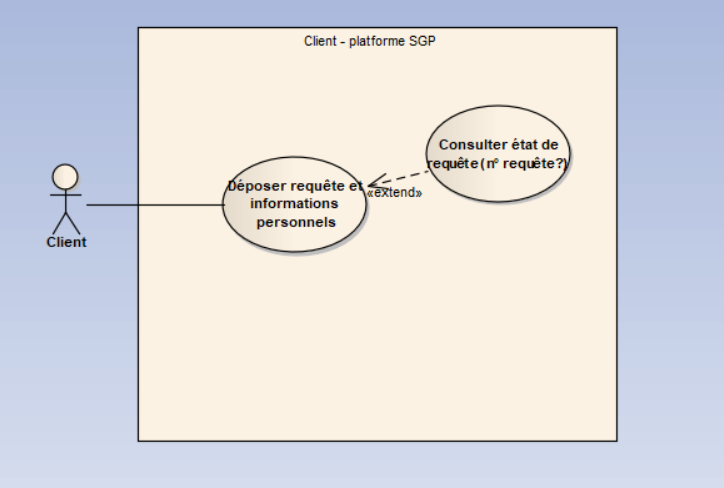
\includegraphics[width=0.92\textwidth]{Figures/GENERAL/Client.png}
    \caption{Cas d'utilisation — Client}
\end{figure}
\textbf{Client — description}
Le client dépose une requête avec ses informations, reçoit un accusé de réception et suit l’état d’avancement jusqu’à décision. Les données alimentent le référentiel et déclenchent la revue par la Direction.

\begin{figure}[H]
    \centering
    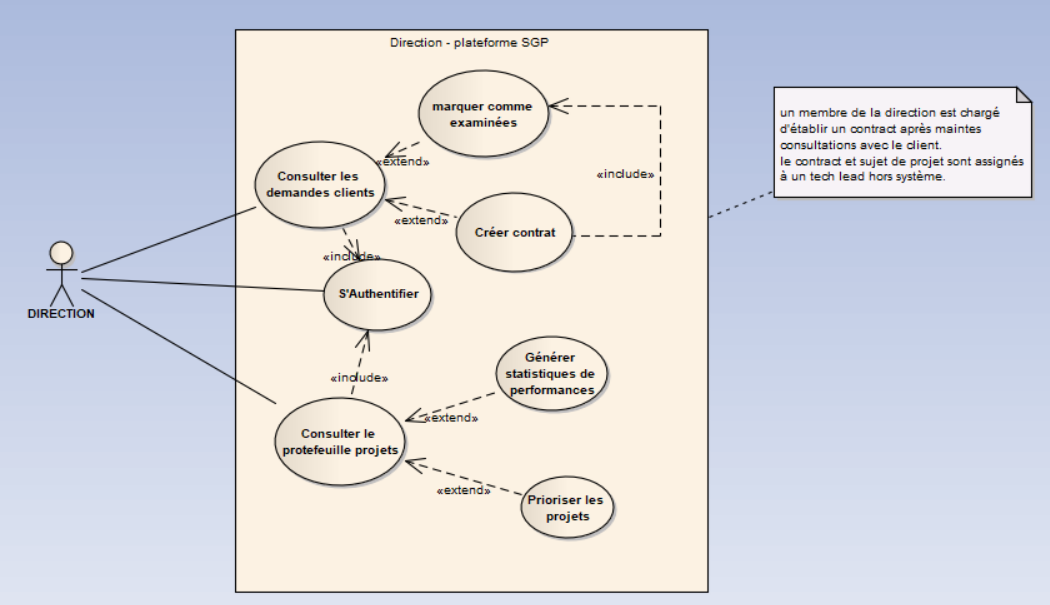
\includegraphics[width=0.92\textwidth]{Figures/GENERAL/Direction.png}
    \caption{Cas d'utilisation — Direction}
\end{figure}
\textbf{Direction — description}
La Direction consulte et marque les demandes, crée les contrats et priorise les projets en s’appuyant sur le portefeuille et les statistiques consolidées.

\begin{figure}[H]
    \centering
    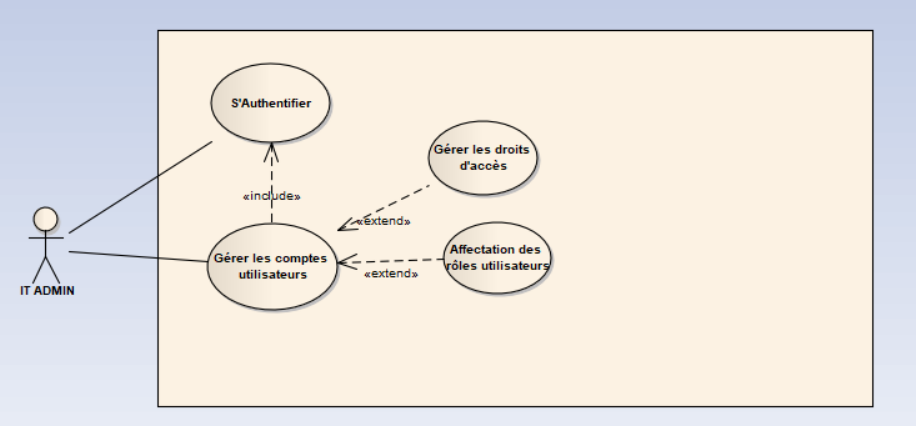
\includegraphics[width=0.92\textwidth]{Figures/GENERAL/ITADMIN.png}
    \caption{Cas d'utilisation — IT Admin}
\end{figure}
\textbf{IT Admin — description}
L’administrateur gère les comptes, les droits d’accès et l’affectation des rôles pour garantir un contrôle d’accès robuste.

% --- Scrum ---
\subsection*{Scrum}
\begin{figure}[H]
    \centering
    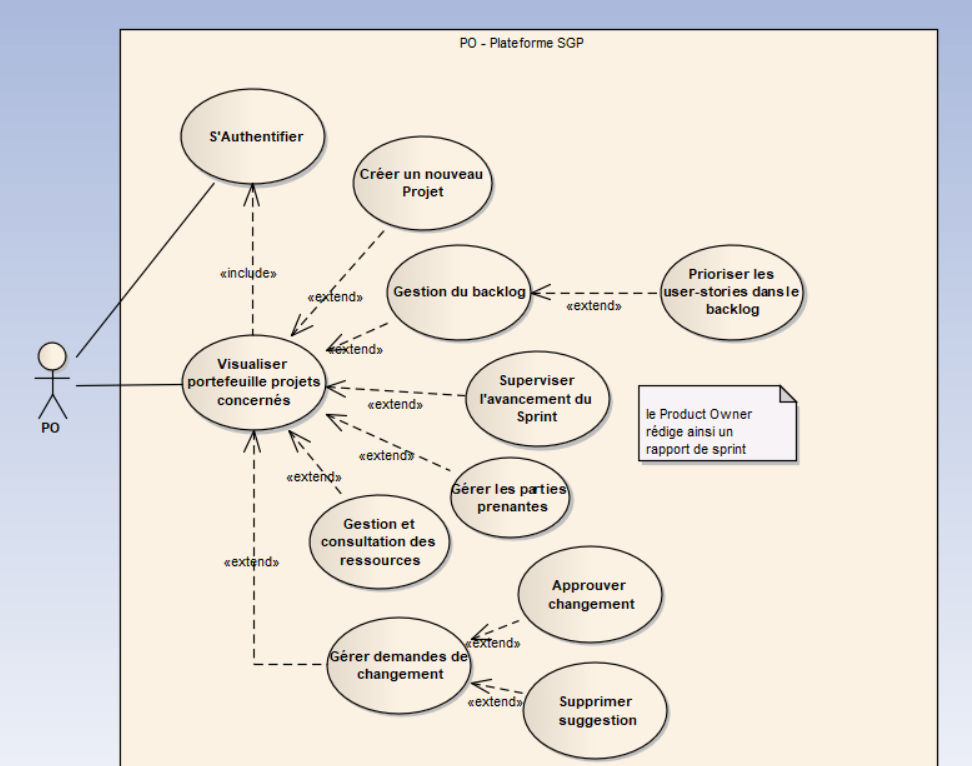
\includegraphics[width=0.92\textwidth]{Figures/SCRUM/PO.png}
    \caption{Cas d'utilisation — Product Owner}
\end{figure}
\textbf{PO — description}
Le PO ordonne le backlog, prépare la planification des sprints, valide les incréments et aligne vision, budget et jalons avec la Direction.

\begin{figure}[H]
    \centering
    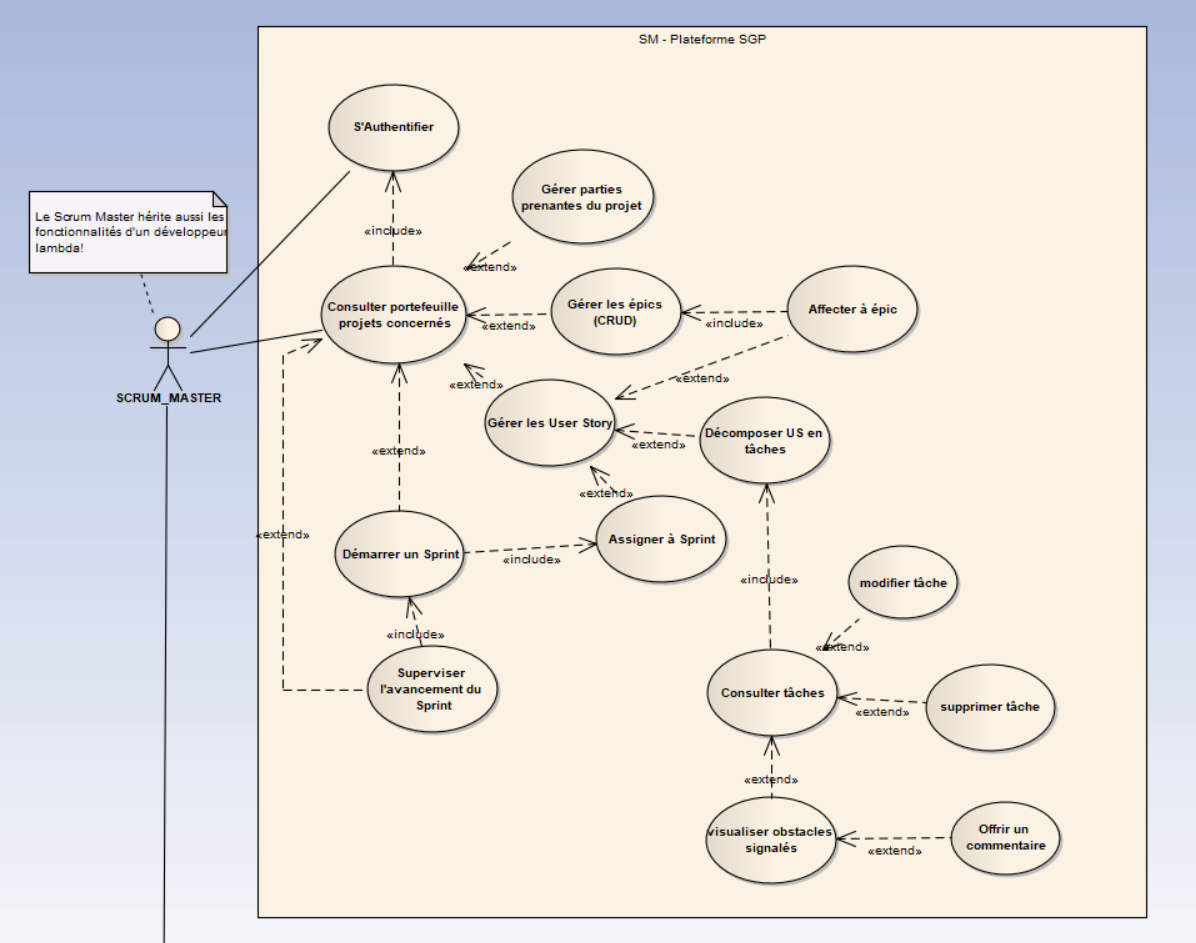
\includegraphics[width=0.92\textwidth]{Figures/SCRUM/SCRUMMASTER.png}
    \caption{Cas d'utilisation — Scrum Master}
\end{figure}
\textbf{Scrum Master — description}
Le SM facilite les rituels, retire les obstacles, suit burndown et vélocité, et coordonne les dépendances inter-équipes.

\begin{figure}[H]
    \centering
    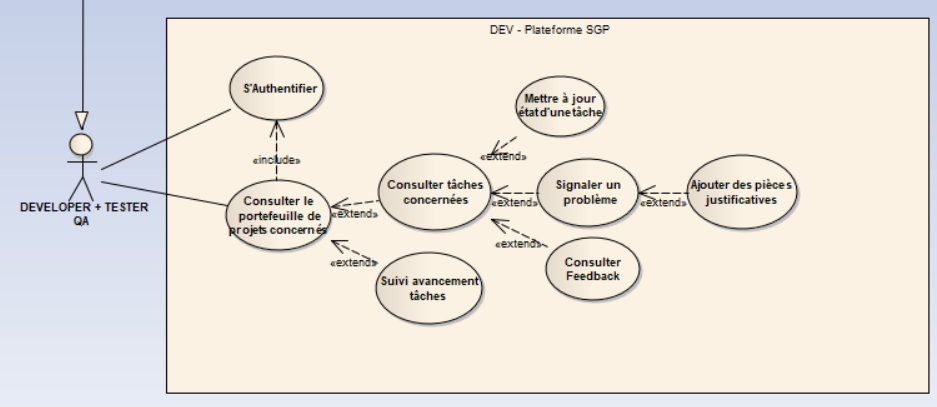
\includegraphics[width=0.92\textwidth]{Figures/SCRUM/DEVTESTERQA.png}
    \caption{Cas d'utilisation — Dev/Tester QA}
\end{figure}
\textbf{Dev/Tester QA — description}
Les membres de l’équipe mettent à jour les tâches, exécutent les tests et consignent le feedback et les pièces justificatives.

% --- Itératif ---
\subsection*{Itératif}
\begin{figure}[H]
    \centering
    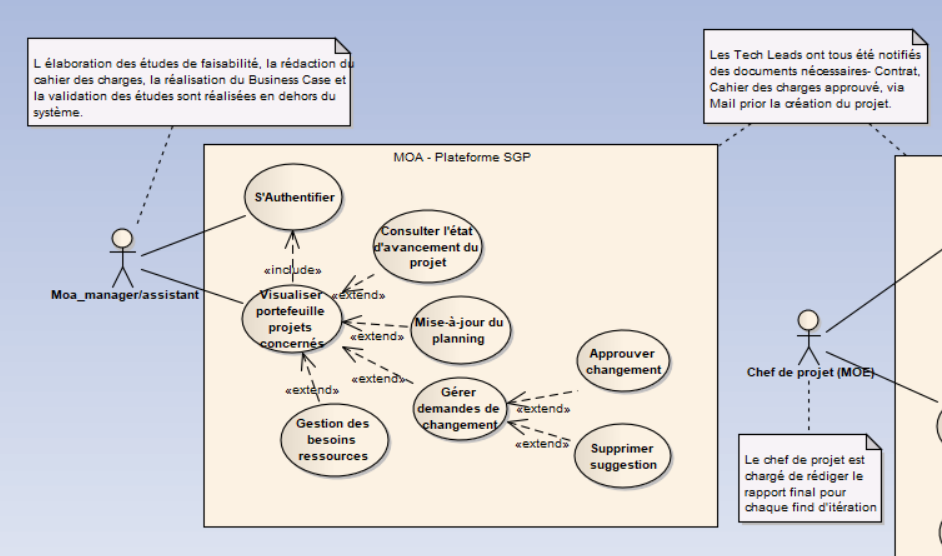
\includegraphics[width=0.92\textwidth]{Figures/ITERATIF/MOA.png}
    \caption{Cas d'utilisation — MOA}
\end{figure}
\textbf{MOA — description}
La MOA pilote la valeur, valide l’avancement et instruit/approuve les demandes de changement.

\begin{figure}[H]
    \centering
    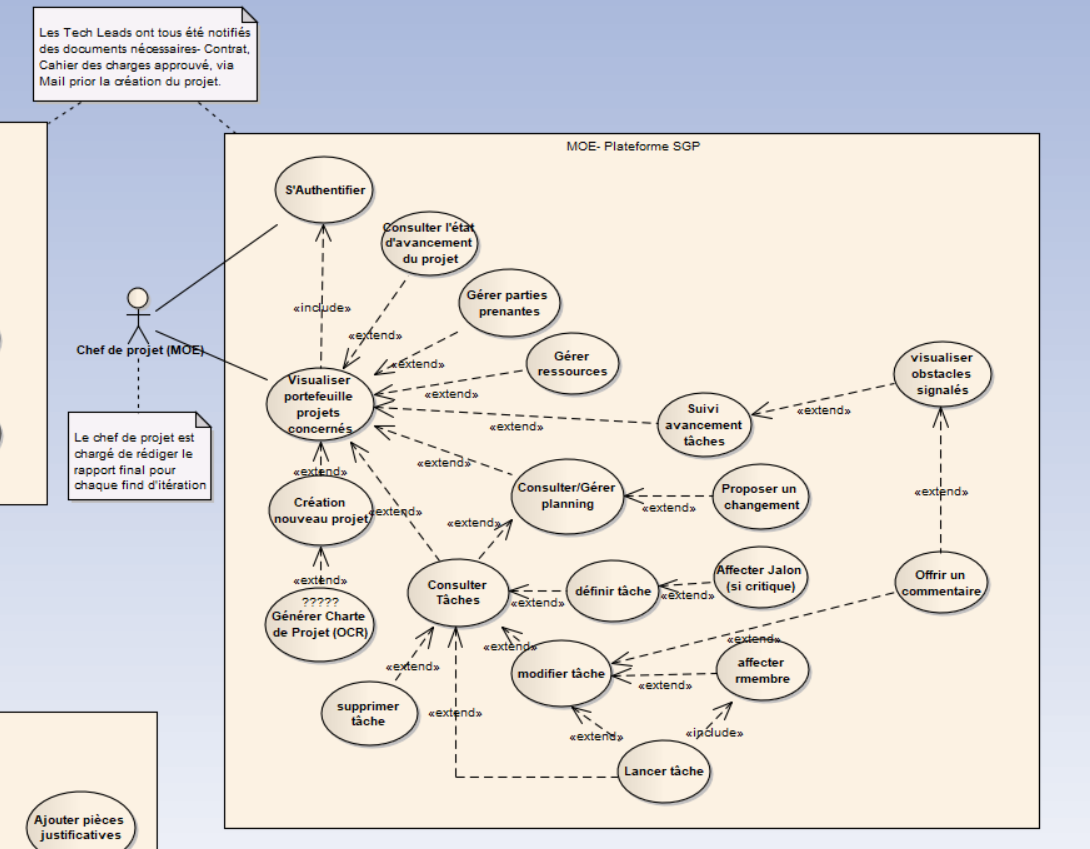
\includegraphics[width=0.92\textwidth]{Figures/ITERATIF/MOE.png}
    \caption{Cas d'utilisation — MOE}
\end{figure}
\textbf{MOE — description}
La MOE structure l’exécution, gère ressources et tâches, synchronise planning et jalons, et analyse l’impact des changements.

\begin{figure}[H]
    \centering
    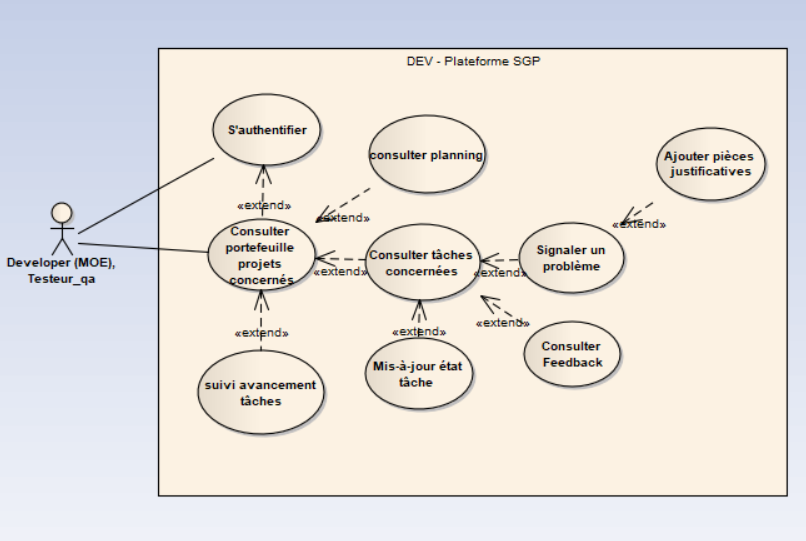
\includegraphics[width=0.92\textwidth]{Figures/ITERATIF/DEV.png}
    \caption{Cas d'utilisation — Dev (itératif)}
\end{figure}
\textbf{Dev (itératif) — description}
Le développeur met à jour l’état des tâches, signale les problèmes et fournit les éléments de preuve pour validation.
% --- Fin section cas d'utilisation détaillés ---

\subsection{Les diagrammes de séquence}
\label{ssec:diagrammes_sequence}

Cette section présente les flux d'interactions dynamiques entre les différents acteurs du système SGP selon deux méthodologies distinctes : Scrum et Itératif. Les diagrammes de séquence suivants décomposent chaque processus en étapes claires, montrant les échanges d'informations entre les acteurs humains et les composants système.

\subsubsection{Processus Scrum}

\begin{figure}[H]
    \centering
    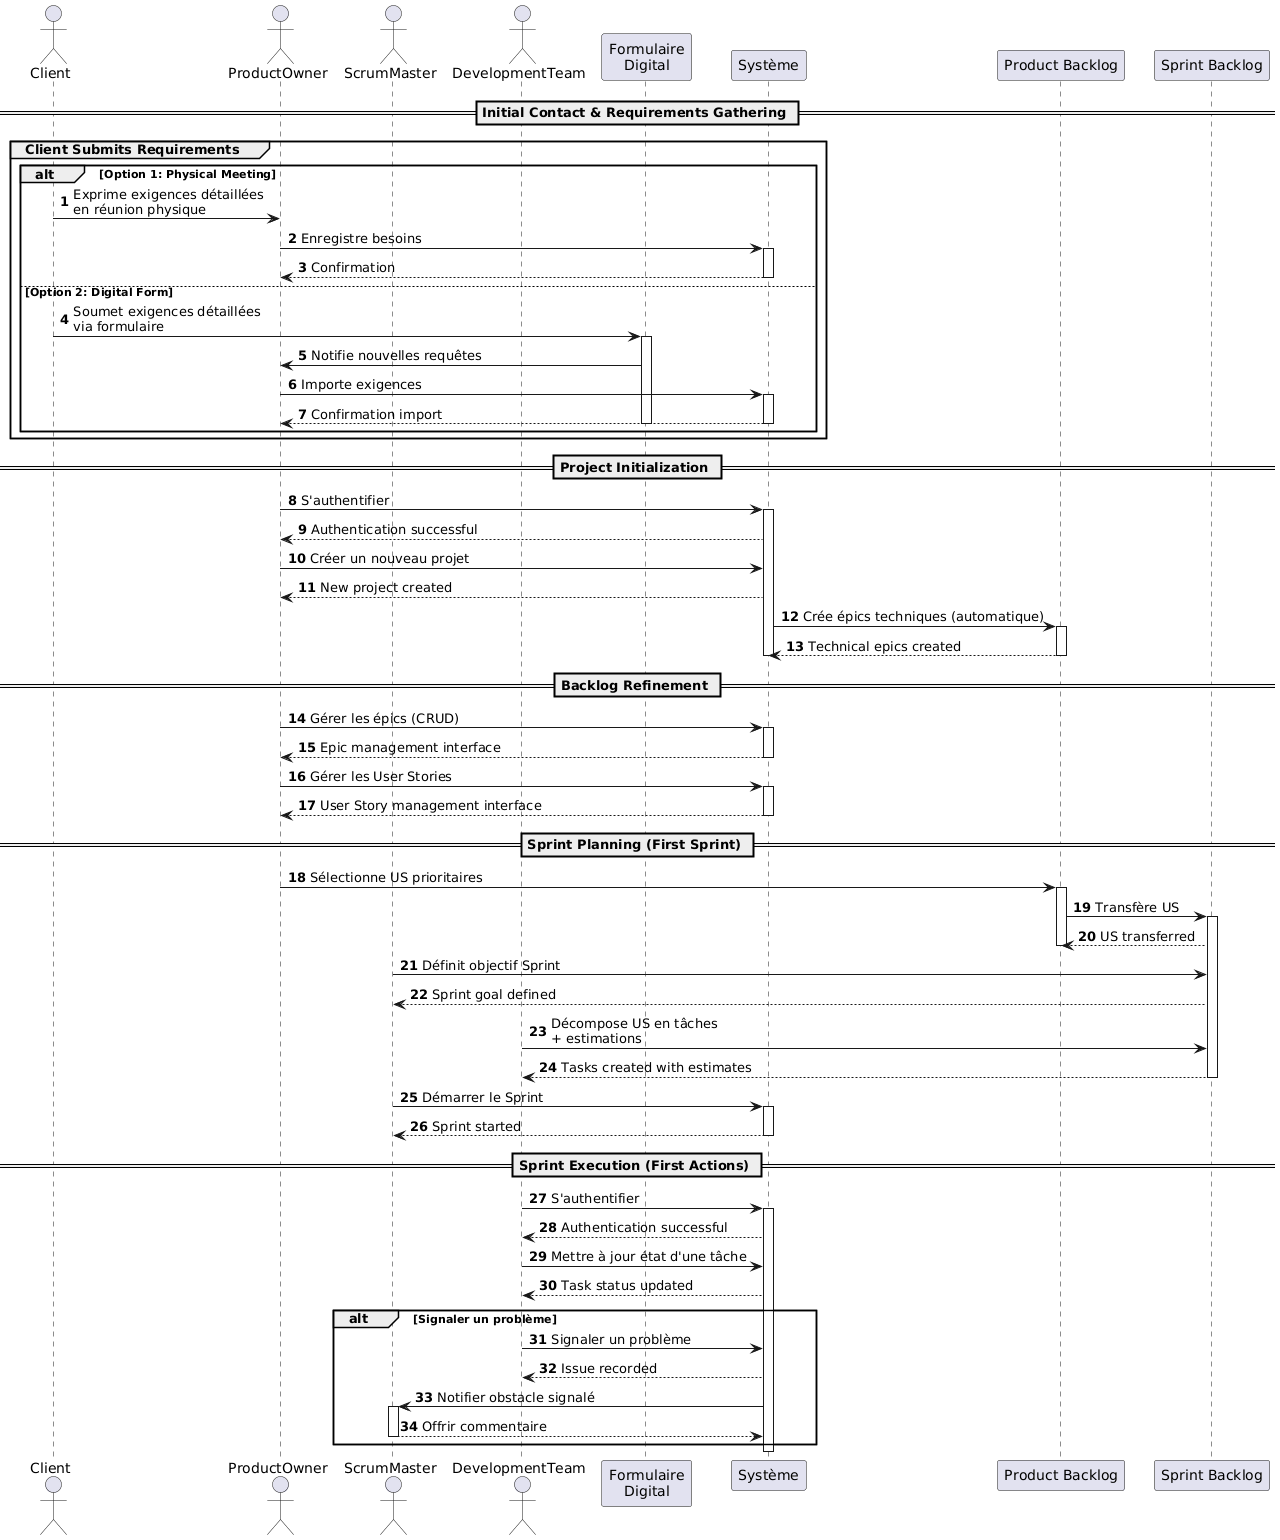
\includegraphics[width=\textwidth]{Figures/SCRUMseq.png}
    \caption{Diagramme de séquence : Processus Scrum}
    \label{fig:seq_scrum}
\end{figure}

\textbf{Processus Scrum (Figure \ref{fig:seq_scrum}) :} Ce diagramme illustre le cycle complet d'un projet Scrum, depuis la collecte des exigences jusqu'à l'exécution des premières actions de sprint. Le processus débute par la soumission des exigences du client, soit via une réunion physique avec le Product Owner, soit via un formulaire digital. Le Product Owner authentifie ensuite le système, crée un nouveau projet et gère les épics techniques automatiquement générés. La phase de raffinement du backlog permet au Product Owner de gérer les épics et les user stories. La planification du premier sprint implique la sélection des user stories prioritaires, leur transfert vers le sprint backlog, la définition de l'objectif du sprint par le Scrum Master, et la décomposition en tâches par l'équipe de développement. L'exécution du sprint commence par l'authentification de l'équipe, la mise à jour des statuts de tâches, et la possibilité de signaler des problèmes avec notification automatique au Scrum Master.

\subsubsection{Processus Itératif}

\begin{figure}[H]
    \centering
    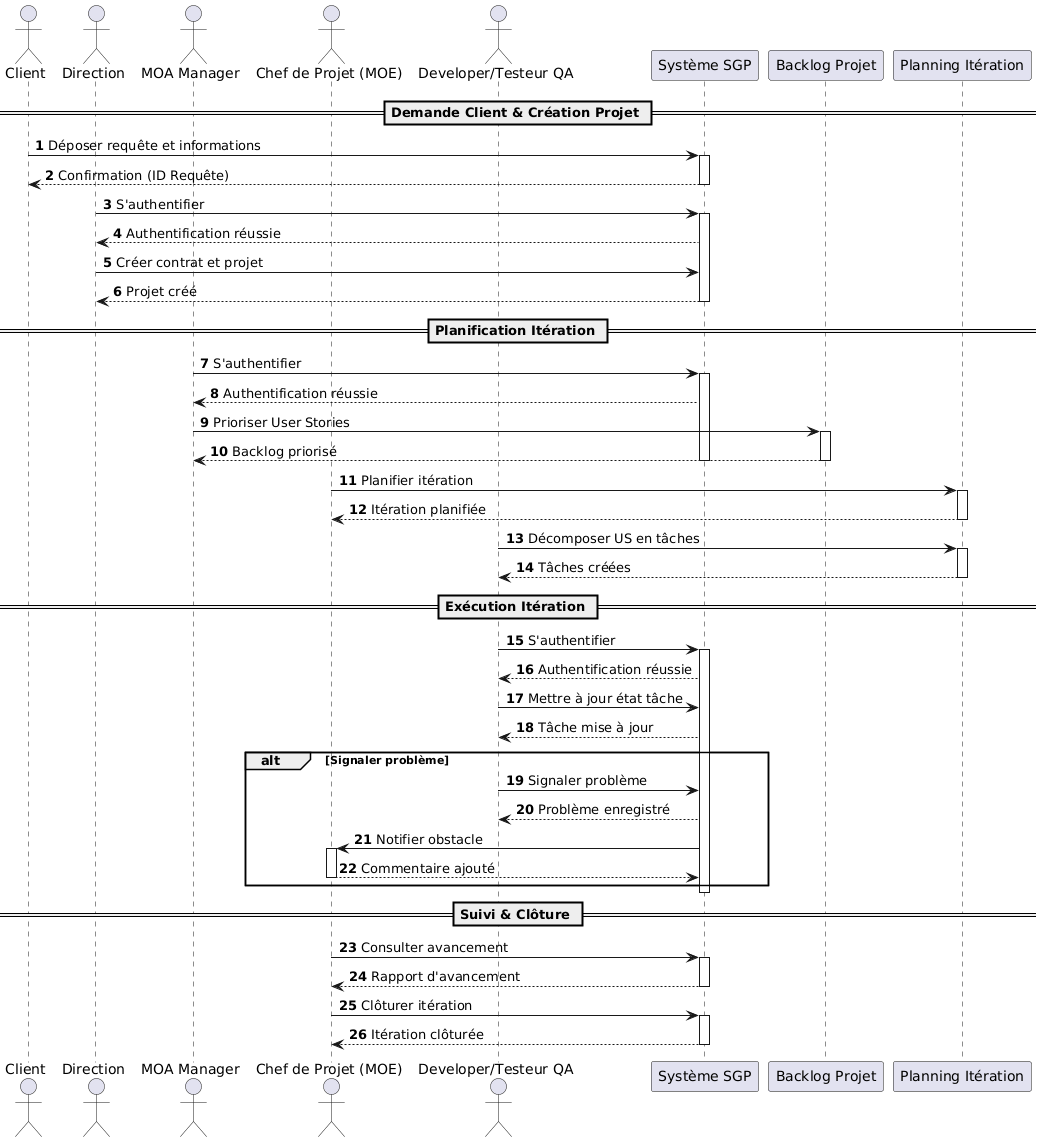
\includegraphics[width=\textwidth]{Figures/ITERATIFseq.png}
    \caption{Diagramme de séquence : Processus Itératif}
    \label{fig:seq_iteratif}
\end{figure}

\textbf{Processus Itératif (Figure \ref{fig:seq_iteratif}) :} Ce diagramme détaille le processus de gestion de projet itératif, structuré en quatre phases principales. La phase de \textbf{demande client et création de projet} commence par le dépôt d'une requête client avec informations détaillées, suivie de l'authentification de la Direction et de la création du contrat et du projet. La phase de \textbf{planification d'itération} implique l'authentification du MOA Manager, la priorisation des user stories dans le backlog projet, la planification de l'itération par le Chef de Projet (MOE), et la décomposition des user stories en tâches par l'équipe de développement. La phase d'\textbf{exécution d'itération} couvre l'authentification de l'équipe, la mise à jour des statuts de tâches, et la gestion des problèmes avec notification automatique au Chef de Projet. Enfin, la phase de \textbf{suivi et clôture} comprend la consultation de l'avancement par le MOA Manager et la clôture formelle de l'itération par le Chef de Projet.


% ===================================================================
% FIN DE LA SECTION : Étude Conceptuelle (VERSION FINALE CORRIGÉE)
% ===================================================================

\section{Conclusion}
\label{sec:conclusion_chap3}

En définitive, la modélisation et l’implémentation réalisées garantissent une solution cohérente, robuste et adaptée aux besoins de gestion. L’utilisation des diagrammes UML et la définition de règles précises ont permis d’assurer la fiabilité et l’intégrité des données. Ce chapitre constitue ainsi une étape clé dans la mise en place d’une plateforme performante et évolutive.